\colorbox{green}{TEMPORARY - CM12}

We have this expression:
$$ \text{P} \subseteq \text{NP} \subseteq \text{PSPACE} \subseteq \text{EXPTIME}$$
However, we do not know if these they are different or not.\\
Order on problems: $S \leq_p T$, where $\leq_p$ is the poly-time reduction.\\

\begin{theorem} 
There is a problem $S \in NP$ such that $\forall T \in NP: T \leq_p S$ 
\end{theorem} 

\begin{figure}[h!]
\centering
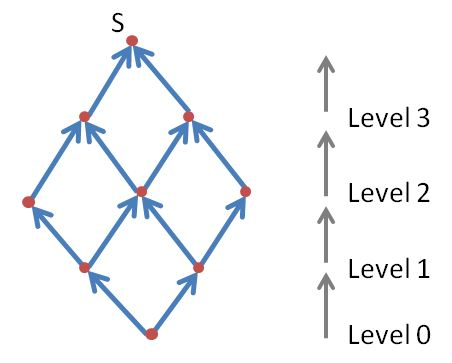
\includegraphics[scale=0.5]{images/fig_1.jpg}
\caption{Reducibility with multiple roots being in fact only one.}
\label{c12:reducibility}
\end{figure}

It is not trivial, we could have the problems reducible for other in many way and
with multiple roots but, in fact, there is only one (see Fig \ref{c12:reducibility} with $\nearrow : \leq_p$: the element which point to the other is the simplest one).

\subsection{SAT Problem}

\begin{definition} SAT problem :
\begin{itemize}
\item Instance: A boolean formula, e.g. $ \left( P \vee \neg Q \right) \wedge Q$, with $\vee$ which corresponds to "or", $\neg$ : "not" and $\wedge$ : "and".
\item Output: Yes, if exists true value for the variables so that the formula evaluates to true, e.g.  \begin{itemize}
\item $\left( P \vee \neg \ Q \right) \rightarrow$ Yes, for P= true
\item $Q \wedge \neg \ Q \rightarrow$ No
\end{itemize}  
\end{itemize}
\end{definition}
\vspace{0.5cm}
\begin{theorem}
$\underbrace{\text{SAT} \in NP \ \ and \ \ \underbrace{\forall T \in NP: T \leq_p \text{SAT}}_{\text{"SAT is NP-hard"}}}_{\text{"SAT is NP-completed"}}$
\end{theorem}

\begin{proof}
(Sketch) 
\begin{itemize}
\item SAT $\in$ NP: certificate= list of TRUE/FALSE values for all variables that make a formula evaluated to YES $\Rightarrow$ ok!
\item  $\forall T \in NP: T \leq_p \text{SAT}$: \\ Let T be in NP, then it exists a Turing Machine M such that $M(x,c)=YES$ for some poly-length certificate c, running in poly-time, if and only if x=YES instance of T.\\
 
We detail the Turing Machine in Fig \ref{c12:turing machine}. 

\begin{figure}[h!]
\centering
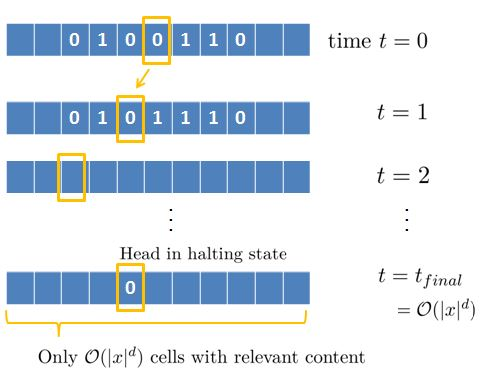
\includegraphics[scale=0.7]{images/fig_2.jpg}
\caption{Turing Machine}
\label{c12:turing machine}
\end{figure}

 $\Rightarrow \mathcal{O}\left( \vert x \vert^{2d} \right)$ variables $P_{t,m}$=TRUE if cell $m$ at time $t$ is 1, with $t$, the time and $m$, the space. $\mathcal{O}\left( \vert x \vert^{d} \right)$ boolean variables describing the head state $P_{t,s}$=TRUE if and only if Head is in state $s$ at time $t$. $\mathcal{O}\left( \vert x \vert^{d} \right)$ variables $Q_{t,m}$=TRUE if and only if head is reading cell $m$ at time $t$. 
 
 We can describe the rules of the Turing Machine by a boolean formula: e.g. $t,m$, the transition $s_1 \longrightarrow s_2$ if we read a $0$. (If $P_{t,s_1}$ and $\neg P_{t,m}$ and $Q_{t,m}$ then $P_{t+1,s_2}$).
 
(Reminder: "If A then B" $\Leftrightarrow \neg A \vee B)$ 

The whole computation is encoded into a big, but poly-size (and computed in poly-time), boolean formula $\phi_{x,c,M}$ (described by $P_{t,m}$ for $t=0\equiv$ Initial state). 

The question "$\exists ? c: T(x,c)=YES$" (for a given $x$). 

Amounts: "Are there truth values for the $P_{0,m}$ encoding $c$ such that $\phi_{x,c,T}$=YES ?", with $x$ and $T$ which are given and $c$ that to be found. 

$\Rightarrow$ This is a SAT-instance 

$\Rightarrow T \leq_{p} $ SAT
\end{itemize} 
\end{proof}

Intuition: SAT is "the hardest" problem in NP \\
The main technique to prove that a problem $S$ is NP-complete is:
\begin{itemize}
\item prove that S $\in$ NP
\item for some other NP-complete problem $S_0$, e.g. $S_0=$SAT, prove that $S_0 \leq_p S$
\end{itemize}
You can conclude:
\begin{itemize}
\item $S$ is NP-complete
\item $S \equiv_p S_0 \equiv$ SAT
\end{itemize}
Since we conjecture that $P\neq NP$, the practical consequence is that we cannot reasonably hope to find a poly-time algorithm for $S$. 
 
\subsection{NP-Complete Problems}

To this day, thousands of interesting problems have been proved NP-complete.

\begin{example}
\begin{leftbar}
$3$ (possibly negated) variables, related by $1$.
\begin{definition}
3-SAP:
\begin{itemize}
\item Instance: A boolean formula in the form $\underbrace{\left( P \vee \neg Q \vee R \right)}_{"clause"} \wedge \left( \neg P \vee \neg R \vee S \right) \wedge \left( P \vee P  \vee Q \right)$. The clauses are linked by $\neg$.
\item Output: YES if satisfiable (i.e. true for some value of $P,Q,R,S,\cdots$) 
\end{itemize}
\end{definition}
\end{leftbar}
\end{example}

\begin{theorem}
3-SAT is NP-complete
\end{theorem}
\begin{proof}
\begin{itemize}
\item 3-SAT $\in$ NP: clear
\item 3-SAT is NP-hard ?, we prove SAT $\leq_p$ 3-SAT
\end{itemize}

The reduction proceeds by transforming in poly-time every boolean formula into the normal form $( \vee \ \ \vee ) \wedge ( \vee \ \ \vee) \wedge \cdots$ using the identities of boolean logic in a systematic way. e.g. : \\
$(P \wedge Q) \vee R \equiv (P \vee R) \wedge (Q \vee R)$ distribution \\
$ \neg (P \vee Q) \equiv \neg P \vee \neg Q$ (de Morgan) and More. 
\end{proof}

3-SAT can help prove that even more problems are NP-complete. 

\subsection{Clique Problem}

\begin{theorem}
CLIQUE is NP-complete
\end{theorem}

\begin{proof}
\begin{itemize}
\item CLIQUE $\in$ NP: certificate of a YES-instance= list of nodes in the CLIQUE
\item CLIQUE is NP-hard ? \\
we show 3-SAT $\leq_p$ CLIQUE.  \\
We have to transform every formula $\phi=\underbrace{( \cdots \vee \cdots \vee \cdots) \wedge ( \cdots ) \wedge ( \cdots)}_{\text{k clauses}}$ into a CLIQUE instance: a graph or an integer. 

We illustrate on an example: \\ $\phi=(\neg x_1 \vee x_2 \vee x_3) \wedge (x_1 \vee \neg x_2 \vee \neg x_3) \wedge (x_1 \vee x_2 \vee x_3) \wedge (x_2 \vee x_3 \vee \neg x_4)$: 4 clauses \\ $f(\phi)=$(Graphe,4)=instance of CLIQUE \ref{c12:clique1}. 

\begin{figure}[h!]
\centering
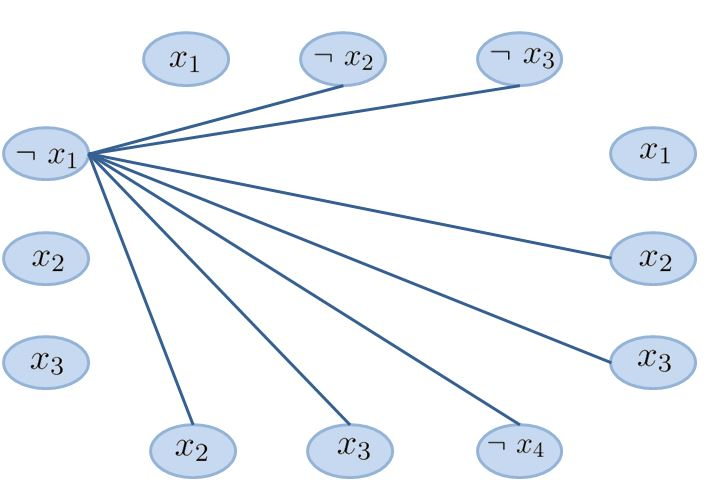
\includegraphics[scale=0.5]{images/fig_3.jpg}
\caption{example of clique}
\label{c12:clique1}
\end{figure}

All pair of nodes are linked except: 
\begin{itemize}
\item inside a triplet representing a clause
\item $x_i$ with $\neg x_i$
\end{itemize}

We check, if $\phi$ is satisfiable then it exists k-clique in the graph. Indeed, if $\phi$ satisfiable by: 

\begin{center}
\begin{tabular}{lll}
$\neg x_1$ &=TRUE in clause & $1$ \\$\neg x_2$ &=TRUE in clause & $2$ \\ $ x_3$ &=TRUE in clause & $3$ \\ $x_4$ &=TRUE in clause & $4$
\end{tabular}
\end{center}

(at least one is true in every clause - see fig \ref{c12:clique2})

\begin{figure}[h!!]
\centering
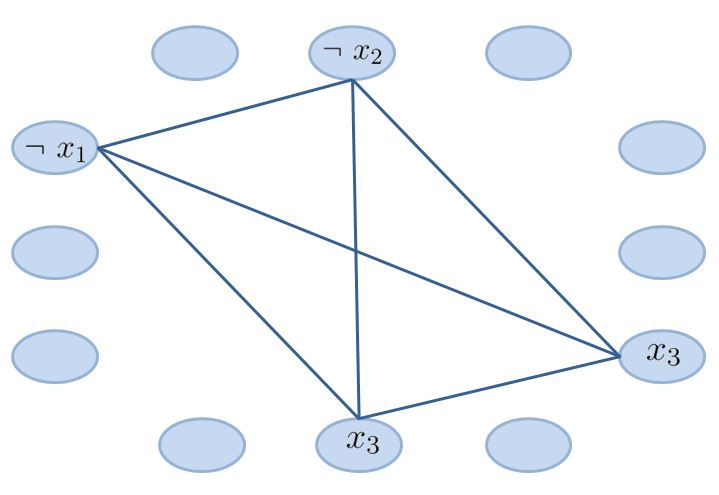
\includegraphics[scale=0.45]{images/fig_4.jpg}
\caption{example of clique}
\label{c12:clique2}
\end{figure}

If there exists k-CLIQUE in a graph then $\phi$ is satifiable.
 Indeed, we find clique then we can see that the assignment : \\
 
 \begin{center}
\begin{tabular}{ccc}
$ \neg x_1$ & =& TRUE \\
$\neg x_2$ & =& TRUE \\
 $x_3$ & =& TRUE \\
 $x_3$ & =& TRUE \\
\end{tabular}
\end{center}
(and anything for other variables) makes $\Phi$ true (because well defined and makes one possibly negated) variable true in every clause.\\
\end{itemize}
\end{proof}

Often practical problems are optimization problems.\\

\begin{definition}
MAX clique:
\begin{itemize}
\item Instance: A graph
\item Output:  Clique of max size
\end{itemize}

We convert this into a decision problem: CLIQUE and we can run CLIQUE for several $k$ (e.g.by dichotomy )
\end{definition}